\documentclass[a4paper, top=10mm]{article}
%for writing from the top
\usepackage{fullpage}
%for math
\usepackage{amsmath}
\usepackage{mathrsfs}
\usepackage{amsthm}
%for images
\usepackage{graphicx}
\usepackage{tikz}
\usepackage{wrapfig}
%for color
\usepackage{xcolor}
%for title
\title{\textbf{\huge{Correct Christmas Tree}}}
\author{Enigma n\textsuperscript{o}5}
\date{14\textsuperscript{th} December 2023}

\newtheorem*{hint}{Hint}

\addtolength{\voffset}{-2cm}
\addtolength{\textheight}{5cm}


\begin{document}
	\maketitle
	
	\begin{wrapfigure}{r}{0.35\textwidth}
		\vspace{-2.5cm}
		\hspace{-0.75cm}
		
\includegraphics[width=1.3\linewidth]{05_xmas_tree.png} 
	\end{wrapfigure}
	
	For a tree triangle to be correct, the numbers in the Christmas bauble need to be equal to the difference of the two bauble below (except on the lowest line, which is free).
	Moreover, the tree must contain natural numbers from $1$ to $n$, $n$ being the total number of baubles in the tree triangle.
	
	You are given the tree triangles of level 1, 2, and 3.
	Complete the tree triangles of level 4 and 5.
	
	
	\begin{center}
		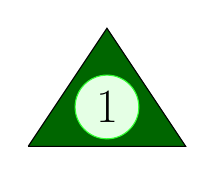
\begin{tikzpicture}
			\filldraw[fill=black!30!green, fill=black!60!green] (0,0.5) -- (1,2) -- (2,0.5) -- (0,0.5);
			\tikzstyle{every node}=[circle,font=\LARGE,draw=green!80,fill=green!10]
			\node at (1,1) {1};
		\end{tikzpicture}
		
		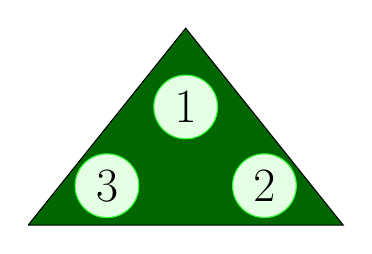
\begin{tikzpicture}
			\filldraw[fill=black!30!green, fill=black!60!green] (-1,-0.5) -- (1,2) -- (3,-0.5) -- (-1,-0.5);
			\tikzstyle{every node}=[circle,font=\LARGE,draw=green!80,fill=green!10]
			\node at (1,1) {1};
			\node at (2,0) {2};
			\node at (0,0) {3};
		\end{tikzpicture}
		
		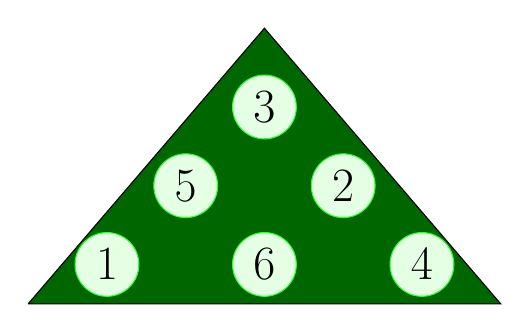
\begin{tikzpicture}
			\filldraw[fill=black!30!green, fill=black!60!green] (-1,-0.5) -- (2,3) -- (5,-0.5) -- (-1,-0.5);
			\tikzstyle{every node}=[circle,font=\LARGE,draw=green!80,fill=green!10]
			\node at (2,2) {3};
			\node at (3,1) {2};
			\node at (1,1) {5};
			\node at (0,0) {1};
			\node at (2,0) {6};
			\node at (4,0) {4};
		\end{tikzpicture}
		
		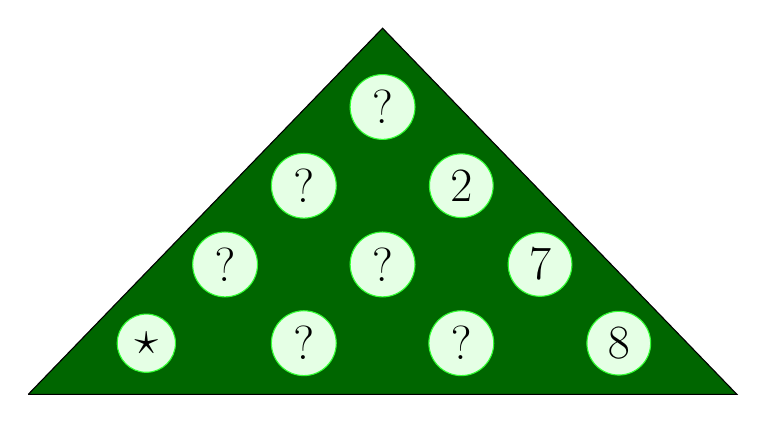
\begin{tikzpicture}
			\filldraw[fill=black!30!green, fill=black!60!green] (-1.5,-0.65) -- (3,4) -- (7.5,-0.65) -- (-1.5,-0.65);
			\tikzstyle{every node}=[circle,font=\LARGE,draw=green!80,fill=green!10]
			\node at (3,3) {?};%3
			\node at (4,2) {2};
			\node at (2,2) {?};%5
			\node at (1,1) {?};%4
			\node at (3,1) {?};%9
			\node at (5,1) {7};
			\node at (0,0) {$\star$};%6
			\node at (2,0) {?};%10
			\node at (4,0) {?};%1
			\node at (6,0) {8};
		\end{tikzpicture}
		
		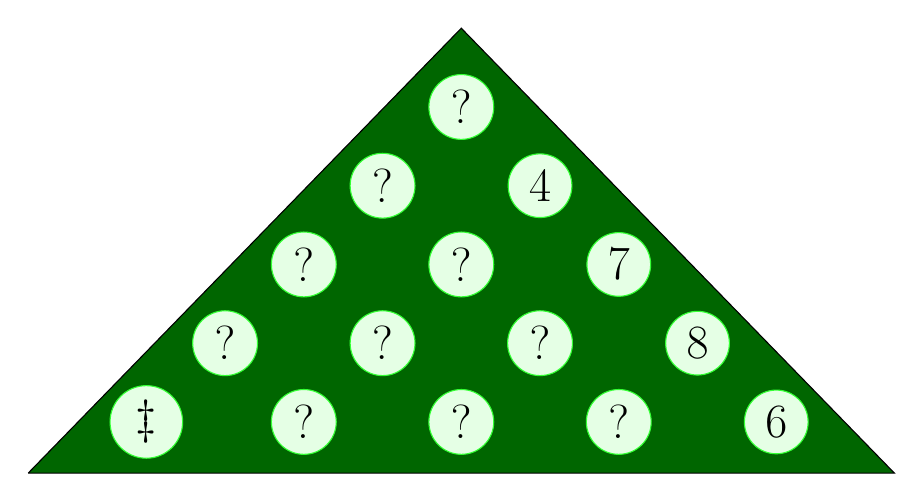
\begin{tikzpicture}
			\filldraw[fill=black!30!green, fill=black!60!green] (-1.5,-0.65) -- (4,5) -- (9.5,-0.65) -- (-1.5,-0.65);
			\tikzstyle{every node}=[circle,font=\LARGE,draw=green!80,fill=green!10]
			\node at (4,4) {?};%5
			\node at (5,3) {4};
			\node at (3,3) {?};%9
			\node at (2,2) {?};%2
			\node at (4,2) {?};%11
			\node at (6,2) {7};
			\node at (1,1) {?};%10
			\node at (3,1) {?};%12
			\node at (5,1) {?};%1
			\node at (7,1) {8};
			\node at (0,0) {$\ddagger$};%13
			\node at (2,0) {?};%3
			\node at (4,0) {?};%15
			\node at (6,0) {?};%14
			\node at (8,0) {6};
		\end{tikzpicture}
	\end{center}
	
	\textbf{What is the value of $\star \ddagger$ ?}
	\textit{(multiplication of $\star$ and $\ddagger$)}
	
\end{document}